\documentclass[crop,tikz]{standalone}

\usetikzlibrary{automata,positioning}

\begin{document}
  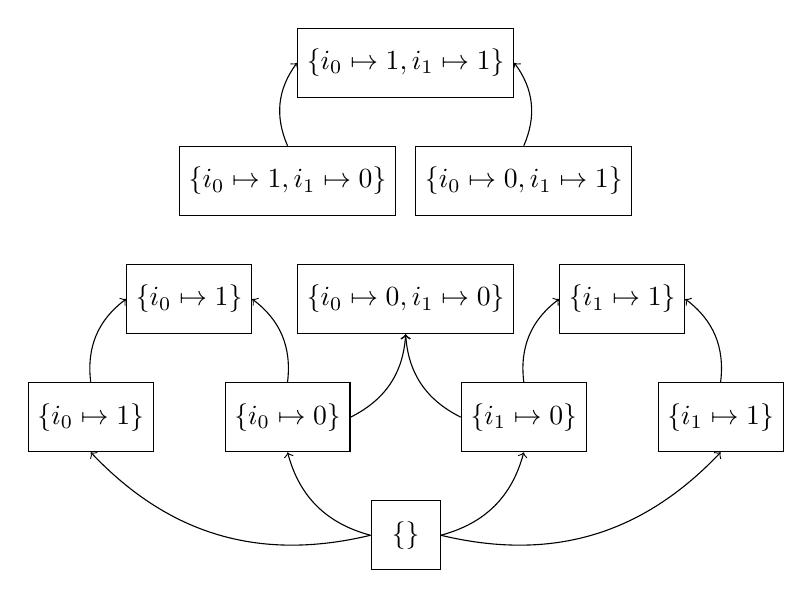
\begin{tikzpicture}
    \node[state,rectangle] (s0) at (0,0) {$\{\}$};
    \node[state,rectangle] (s1) at (-1.5, 1.5) {$\{ i_0 \mapsto 0 \}$};
    \node[state,rectangle] (s3) at (-4, 1.5) {$\{ i_0 \mapsto 1 \}$};
    \node[state,rectangle] (s5) at (-2.75, 3) {$\{ i_0 \mapsto 1 \}$};
    \node[state,rectangle] (s2) at (1.5, 1.5) {$\{ i_1 \mapsto 0 \}$};
    \node[state,rectangle] (s4) at (4, 1.5) {$\{ i_1 \mapsto 1 \}$};
    \node[state,rectangle] (s6) at (2.75, 3) {$\{ i_1 \mapsto 1 \}$};
    \node[state,rectangle] (s7) at (0, 3) {$\{ i_0 \mapsto 0, i_1 \mapsto 0 \}$};
    \node[state,rectangle] (s8) at (-1.5, 4.5) {$\{ i_0 \mapsto 1, i_1 \mapsto 0 \}$};
    \node[state,rectangle] (s9) at (1.5, 4.5) {$\{ i_0 \mapsto 0, i_1 \mapsto 1 \}$};
    \node[state,rectangle] (s10) at (0, 6) {$\{ i_0 \mapsto 1, i_1 \mapsto 1 \}$};

    % \node[state] (A) [] {$A$};
    % \node[state] (B) [right = of A] {$B$};
    % \node[state] (C) [right = of B] {$C$};
    % \node[state] (D) [right = of C] {$D$};
    % \node[state] (E) [below = of A] {$E$};
    % \node[state] (F) [right = of E] {$F$};
    % \node[state] (G) [right = of F] {$G$};
    % \node[state] (H) [right = of G] {$H$};

    \path[->] (s0.west) edge [bend left] node [] {} (s1.south);
    \path[->] (s0.west) edge [bend left] node [] {} (s3.south);
    \path[->] (s0.east) edge [bend right] node [] {} (s2.south);
    \path[->] (s0.east) edge [bend right] node [] {} (s4.south);
    \path[->] (s3.north) edge [bend left] node [] {} (s5.west);
    \path[->] (s1.north) edge [bend right] node [] {} (s5.east);
    \path[->] (s4.north) edge [bend right] node [] {} (s6.east);
    \path[->] (s2.north) edge [bend left] node [] {} (s6.west);
    \path[->] (s1.east) edge [bend right] node [] {} (s7.south);
    \path[->] (s2.west) edge [bend left] node [] {} (s7.south);
    \path[->] (s8.north) edge [bend left] node [] {} (s10.west);
    \path[->] (s9.north) edge [bend right] node [] {} (s10.east);
    % \path[-] (B) edge node [above] {$2$} (C);
    % \path[-] (C) edge node [left] {$2$} (G);
    % \path[-] (A) edge node [left] {$4$} (E);
    % \path[-] (F) edge node [above] {$1$} (G);
    % \path[-] (G) edge node [above left] {$1$} (D);
    % \path[-] (G) edge node [above] {$1$} (H);
  \end{tikzpicture}
\end{document}
